\section{Introduction}
I have spent the majority of my time this week testing the Spearman Rank correlation, Topological idea and grasping the idea of AMNet\cite{amnet} by Jiri Fajtl.

\section{Spearman Rank Correlation Experiments}
This week I tested the Spearman Rank Correlation computation on ground-truth and some values inherited from the groundtruth itself.

\textbf{\emph{Keep the Groundtruth by itself}}. I calculated the correlation between the groundtruth and itself to validate my reasoning that it would be 1. These were the results; \textbf{\emph{Spearman's Correlation}} value of \textbf{\emph{1.0}}, \textbf{\emph{Pearson's Correlation}} value of \textbf{\emph{1.0}}, \textbf{\emph{Mean Squared Error}} value of \textbf{\emph{0.0}}.

\textbf{\emph{Divide the Groundtruth by 2}}. I divided the groundtruth by 2 and calculated the correlation between them. These were the results; \textbf{\emph{Spearman's Correlation}} value of \textbf{\emph{1.0}}, \textbf{\emph{Pearson's Correlation}} value of \textbf{\emph{1.0}}, \textbf{\emph{Mean S-quared Error}} value of \textbf{\emph{0.16}}.

\textbf{\emph{Ordinal Ranking}}. For example I had 6 elements \textbf{\emph{[0.45, 0.25, 0.1, 0.2, 0.25, 0.15]}}, the ordinal ranking of these 6 elements would be \textbf{\emph{[6, 4, 1, 3, 5, 2]}}. This ranking technique did not care about equal values, it just ranked the elements by their values and their index (for equal values). I calculated the correlation between the groundtruth and its ordinal ranking. These were the results; \textbf{\emph{Spearman's Correlation}} value of \textbf{\emph{0.999}}, \textbf{\emph{Pearson's Correlation}} value of \textbf{\emph{0.966}}, \textbf{\emph{Mean Squared Error}} value of \textbf{\emph{21319943.72}}. Because the ranks were far from the groundtruth so it was reasonable for the mean squared error value to be a huge number.

\textbf{\emph{Max Ranking}}. Given 6 elements as the example above, the max ranking of these 6 elements would be \textbf{\emph{[6, 5, 1, 3, 5, 2]}}. This ranking technique based on the ordinal ranking, but it treated equal values as the same ranks and their ranks would be the maximum one in term of their ordinal ranks. I calculated the correlation between the groundtruth and its max ranking. These were the results; \textbf{\emph{Spearman's Correlation}} value of \textbf{\emph{1.0}}, \textbf{\emph{Pearson's Correlation}} value of \textbf{\emph{0.968}}, \textbf{\emph{Mean Squared Error}} value of \textbf{\emph{22609763.39}}. As this ranks also made the predict results completely differed from the groundtruth so the mean squared error was also a huge number.

\textbf{\emph{Dense Ranking}}. Given 6 elements as the example above, the dense ranking of these 6 elements would be \textbf{\emph{[5, 4, 1, 3, 4, 2]}}. This ranking technique treated equal values as the same ranks and kept moving on without making any gaps in the ranking sequence. I calculated the correlation between the groundtruth and its dense ranking. These were the results; \textbf{\emph{Spearman's Correlation}} value of \textbf{\emph{1.0}}, \textbf{\emph{Pearson's Correlation}} value of \textbf{\emph{0.992}}, \textbf{\emph{Mean Squared Error}} value of \textbf{\emph{12969.23}}. Because this ranking technique did not create any gaps so it was much more efficient (in term of memory) and the mean squared error was also smaller than the 2 ranking techniques' above.

After testing these ranking techniques I had a conclusion that the \textbf{\emph{Dense Ranking}} would work best because its Pearson's Correlation value was higher and mean squared error value was much smaller than 2 other ranking techniques above. So it would be a reasonable choice for the Topological Sort idea which would be presented next.

\section{Topological Sort Network}
\subsection{Architecture}
This was actually my mentor's idea and I also confirmed its feasibility after experiments on the Spearman Rank Correlation computation above. My network took in 2 videos at once, concatenated them and pass through several Fully-connected layers to get determine which video was more memorabible than the other one. After comparing all two-video pairs I would use Topological Sort algorithm to retrieve the ranking sequence. Spearman Rank Correlation would be calculated on this ranking sequence and the groundtruth.

\subsection{Training on Dev-Set (extracted by ResNet50)}
\subsubsection{Strategy}
I splitted the provided Dev-Set for this challenge into three parts, since the Dev-Set had 8000 videos, I picked \textbf{\emph{6000}} videos for training, \textbf{\emph{1000}} videos for validating and the last \textbf{\emph{1000}} videos for testing.

\subsubsection{Version 1}
In this version I used 2 hidden layers which size were \textbf{\emph{2048}} and \textbf{\emph{128}}, I also added 3 dropout layers (probability of \textbf{\emph{0.75}} each) between each Fully-connected layers. The figure below demonstrated my version 1 network.

\begin{figure}[!ht]
\centering
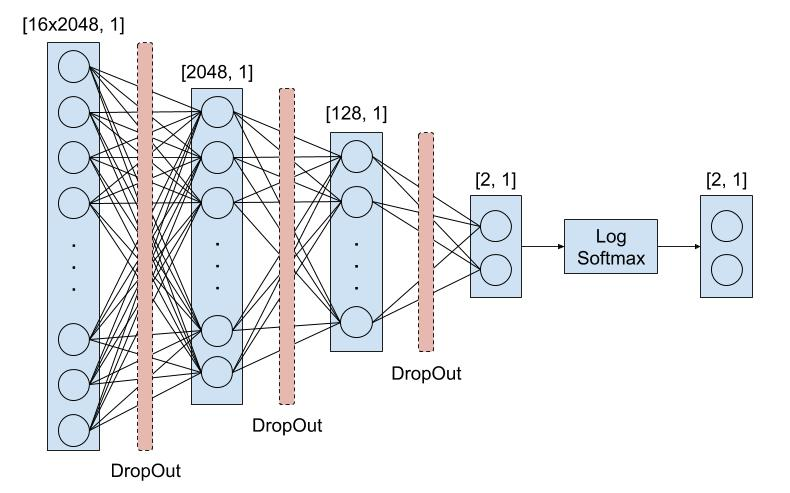
\includegraphics[width=\textwidth]{week12-topological-v1.jpg}
\caption{Topological Sort Network Network Architecture.}
\end{figure}

I trained this network with \textbf{\emph{1000}} epochs. Each epoch I randomly picked a batch of \textbf{\emph{128}} videos and compared each video with others (it meant I had average \textbf{\emph{16384}} comparisons each epoch). The loss value after 1000 epochs was \textbf{\emph{0.078}} and the highest validate accuracy was \textbf{\emph{54.68\%}}.

\begin{figure}[!ht]
\centering
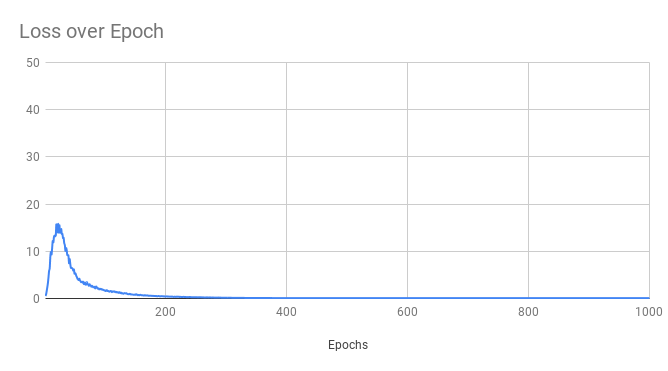
\includegraphics[width=\textwidth]{week12-topological-v1-loss.png}
\caption{Loss over Epoch (on Train set).}
\end{figure}

\begin{figure}[!ht]
\centering
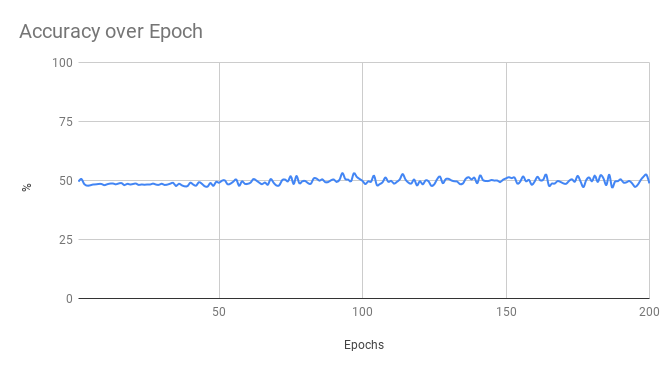
\includegraphics[width=\textwidth]{week12-topological-v1-accuracy.png}
\caption{Accuracy over Epoch (on Validate set).}
\end{figure}

Then I used this trained model to calculate all comparisons between videos and used those values for Topological Sort algorithm to get the final ranking sequence. But the Spearman Rank correlation value was only \textbf{\emph{0.01}}. So I thought this idea was not a reasonable approach.

\newpage
\section{AMNet}
\subsection{Introduction}
In this paper the authors presented the design and evaluation of an end-to-end trainable, deep neural network with a visual attention mechanism for memorability estimation in still images. The author analyzed the suitability of transfer learning of deep models from image classification to the memorability task. Further on the authors studied the impact of the attention mechanism on the memorability estimation and evaluate their network on the SUN Memo-rability and the LaMem datasets. Their network outperforms the existing state of the art models on both datasets in terms of the Spearman’s rank correlation as well as the mean squared error, closely matching human consistency.

\begin{figure}[!ht]
\centering
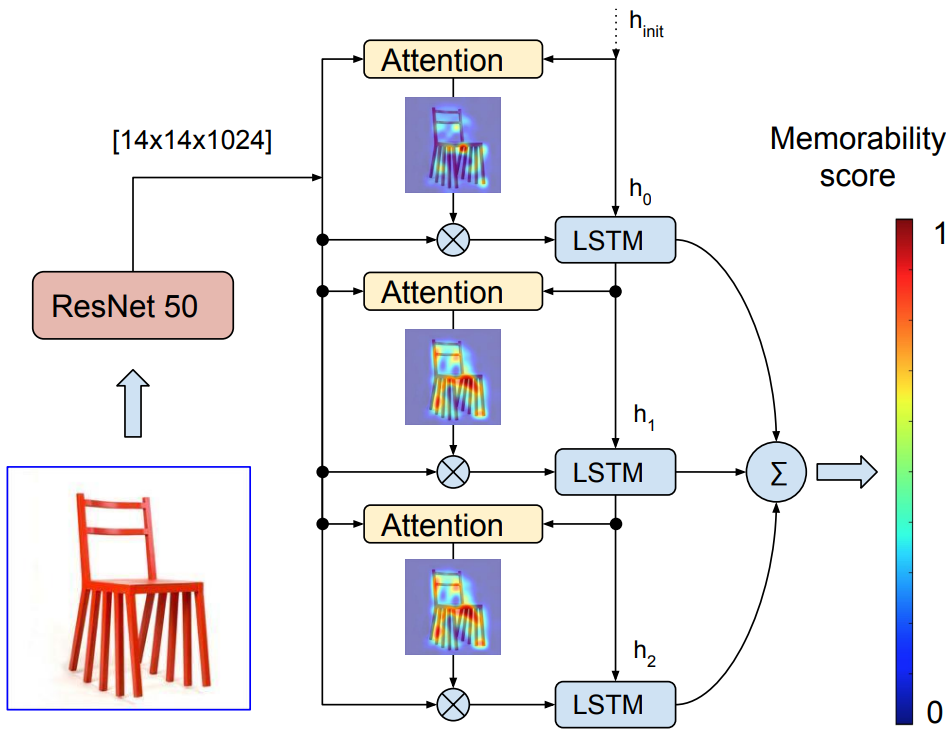
\includegraphics[width=0.9\textwidth]{week12-amnet-general.png}
\caption{AMNet iteratively generates attention maps linked to the image regions correlated with the memorability. After three iterations the memo-rability scores were added and presented on the output.}
\end{figure}

The AMNet estimated the image memorability by taking a single image \textbf{\emph{X}} and generating a memorability score \textbf{\emph{y}}. The process of memorability estimation was summarized in algorithm presented in the figure above. The authors pro-posed all required mathematical equations (Eq.3, Eq.4, Eq.6, ...) in their paper for implement purpose. The figure below demonstrated the detailed process of memorability estimation.

\newpage
\begin{figure}[!ht]
\centering
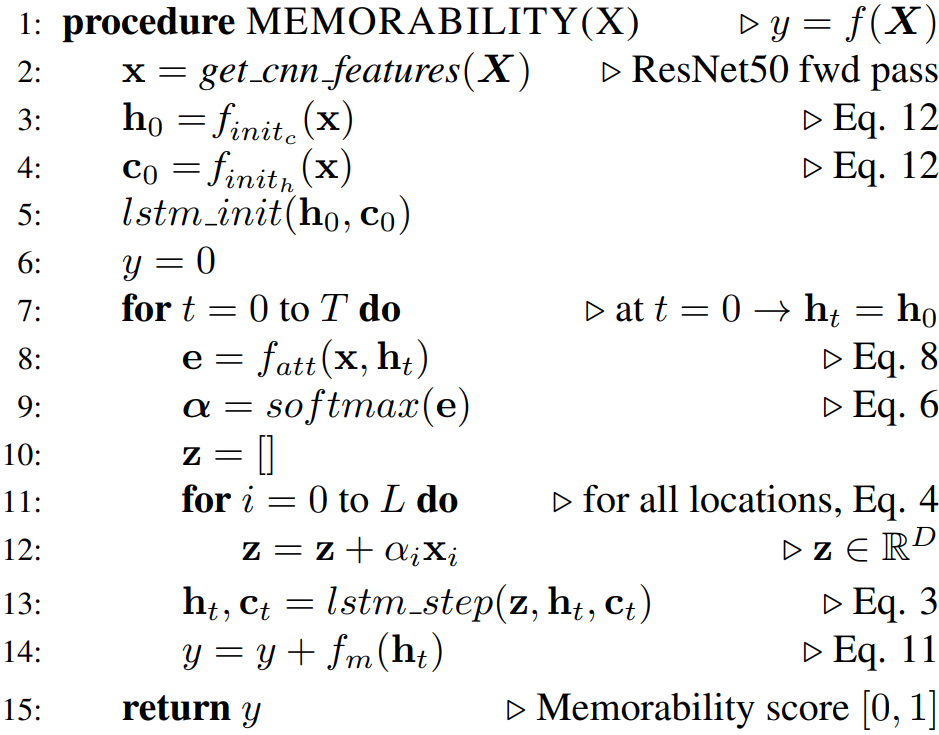
\includegraphics[width=0.6\textwidth]{week12-amnet-algorithm.png}
\caption{Summarized AMNet Algorithm.}
\end{figure}

The authors also proposed their custom loss function in their paper. Their loss function composed of two terms. The first term represented the mean squared error between the groundtruth and predicted image memorability. In order to encourage the attention model to explore all image regions over all time steps, the authors added a second term which performed a joint penalty as a function of activations of all attention maps in the LSTM sequence, which was already introduced by Kelvin Xu\cite{visualatt}.

\begin{figure}[!ht]
\centering
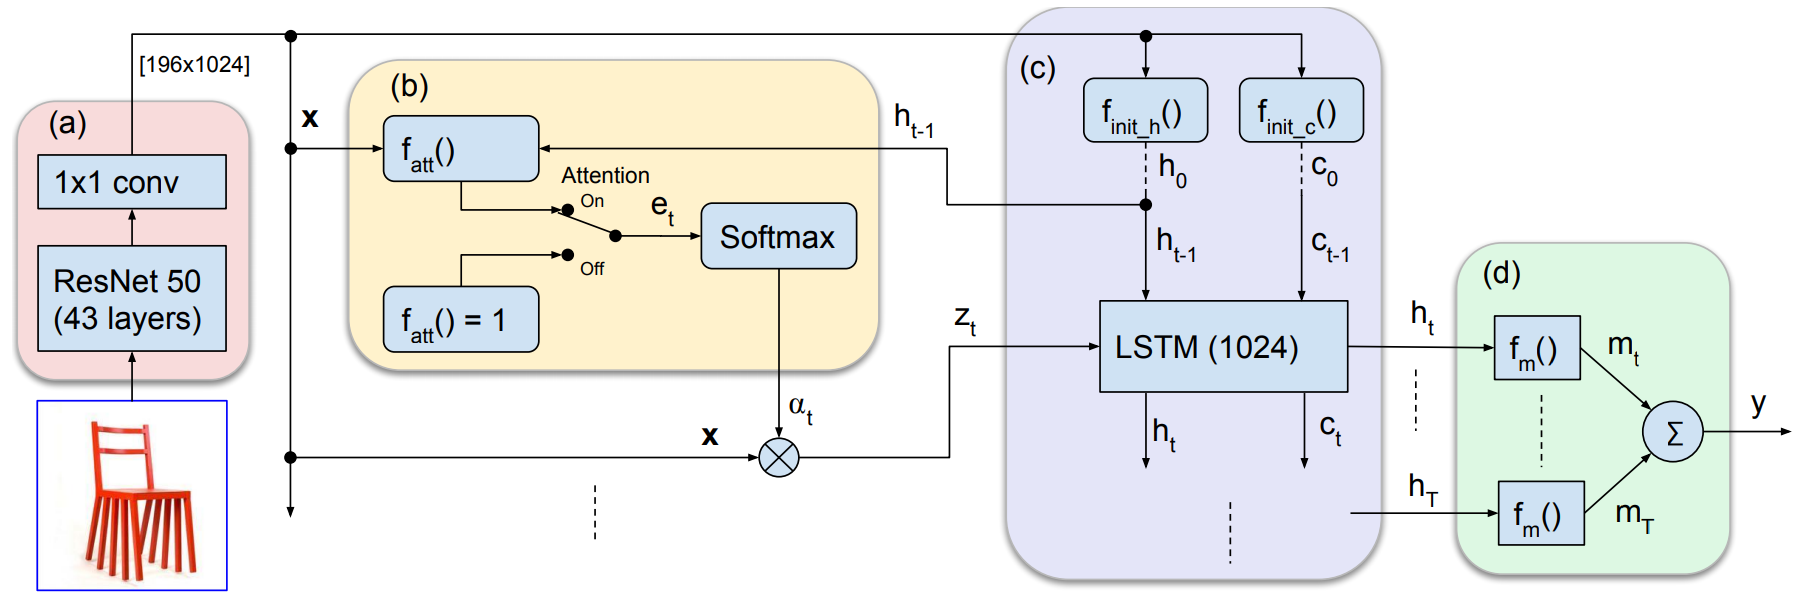
\includegraphics[width=\textwidth]{week12-amnet-detailed.png}
\caption{Detailed AMNet Algorithm.}
\end{figure}

The authors claimed that the entire model was fully differentiable and train-ed end-to-end with the ADAM\cite{adam} optimizer with a fixed learning rate $10^{−3}$. The input image feature vector was extracted from the $43^{rd}$ layer of the RestNet50 with dimensions [14 $\times$ 14 $\times$ 1024]. The ResNet50 was trained for image classification on the ImageNet dataset and its weights were not updated during the AMNet training.

\subsection{Training on LaMem-Set (extracted by Inceptionv3)}
\subsubsection{Strategy}
Instead of using the input image feature vector of dimensions [14 $\times$ 14 $\times$ 1024] and having the sequence length of 14 $\times$ 14 as AMNet, I used the input image feature vector of dimensions [1 $\times$ 2048] and my sequence length was 1. I did not want to complicate my loss function, I just used the mean squared error only. I splitted the LaMem-Set for into two parts, the total number of images was \textbf{\emph{55000}}, I picked \textbf{\emph{45000}} images for training, and \textbf{\emph{10000}} images testing.

\subsubsection{Version 1}
In this version I had my input size of \textbf{\emph{2048}}, hidden size of \textbf{\emph{1024}}, \textbf{\emph{3}} stacking LSTM layer and as mentioned above, my sequence length of \textbf{\emph{1}}. My ADAM optimizer's learning rate was \textbf{\emph{1e-4}}. I trained this version with \textbf{\emph{200}} epochs and saved the snapshot which had the highest correlation value on test set. The loss and the correlation both behaved stably.

\begin{figure}[!ht]
\centering
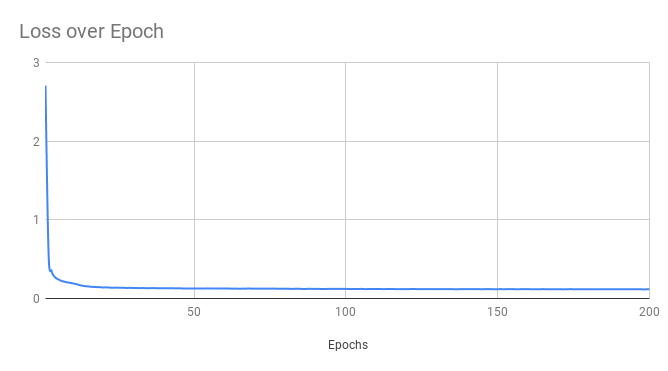
\includegraphics[width=\textwidth]{week12-amnet-lamem-v1-loss.png}
\caption{Loss over Epoch (on Train set).}
\end{figure}

\begin{figure}[!ht]
\centering
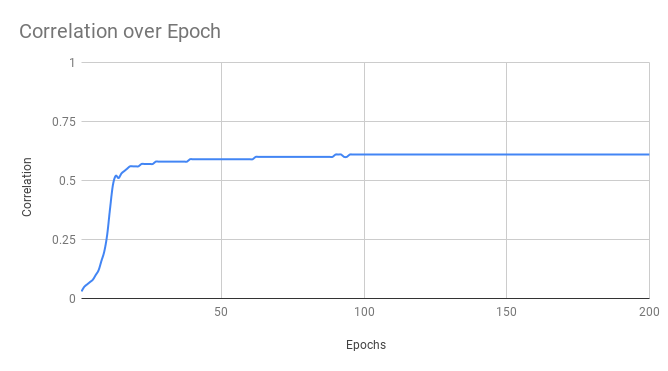
\includegraphics[width=\textwidth]{week12-amnet-lamem-v1-correl.png}
\caption{Correlation over Epoch (on Test set).}
\end{figure}

The loss and correlation value stopped significantly changing from the epoch $100^{th}$ so I thought it only needed 100 epochs to converge. After 200 epochs, my loss was about \textbf{\emph{0.117}} and my final correlation value on test set was \textbf{\emph{0.61}}.

Later, I used this pre-trained model to calculate the correlation value on the Dev-Set but predictably, the result was absolutely terrible, it was not even a positive number.

\subsection{Training on Dev-Set (extracted by ResNet50)}
\subsubsection{Strategy}
I used the same input strategy as the previous version that I trained on LaMem-Set. I also try to conduct the same loss function as the one proposed by the authors which was a combination of mean squared error and attention penalty. I splitted the provided Dev-Set for this challenge into three parts, since the Dev-Set had 8000 videos, I picked \textbf{\emph{6000}} videos for training, \textbf{\emph{1000}} videos for validating and the last \textbf{\emph{1000}} videos for testing.

\subsection{Version 1}
I kept the input size and hidden size as the same as the previous version that I trained on LaMem-Set. This times I changed the number of stacking LSTM layer to \textbf{\emph{1}} and the sequence length to \textbf{\emph{8}}. There was one new hyper-parameter gamma which specified the impact of the attention penalty. I used its value of \textbf{\emph{1e-3}}. Finally was the ADAM optimizer with learning rate of \textbf{\emph{1e-4}}.

After 













